   \begin{center}
        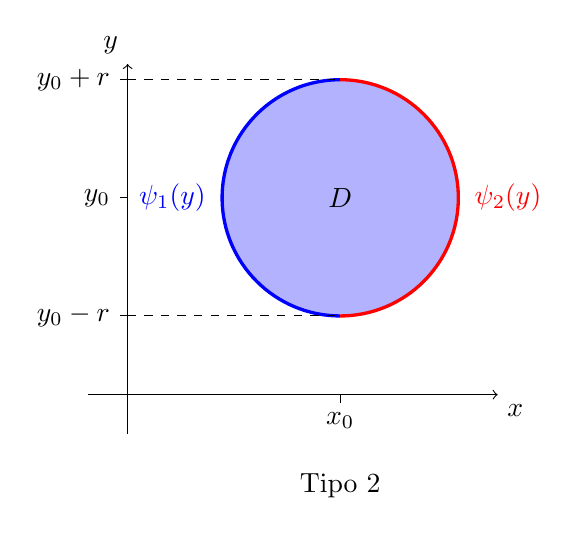
\begin{tikzpicture}
     \begin{scope}[xshift=7cm]
        \def\cxx{2.7}
        \def\cx{2}    % x_0
        \def\cy{2.5}    % y_0
        \def\rr{1.5}  % r

        % ejes
        \draw[->] (-0.5,0) -- (4.7,0) node[below right] {$x$};
        \draw[->] (0,-0.5) -- (0,4.2) node[above left]  {$y$};

        % relleno del círculo
        \fill[blue!30] (\cxx,\cy) circle [radius=\rr];

        % semicircunferencia izquierda: psi_1(y) = -sqrt(r-(y-y0)^2)+x0
        \draw[blue, very thick] (\cxx,\cy-\rr) arc[start angle=270, end angle=90, radius=\rr]
            node[midway, left, xshift=-2pt] {\color{blue}$\psi_1(y)$};
        % semicircunferencia derecha: psi_2(y) = +sqrt(r-(y-y0)^2)+x0
        \draw[red, very thick] (\cxx,\cy-\rr) arc[start angle=-90, end angle=90, radius=\rr]
            node[midway, right, xshift=2pt] {\color{red}$\psi_2(y)$};

        % líneas punteadas horizontales en y_0 - r y y_0 + r
        \draw[dashed] (0,\cy-\rr) -- (\cxx,\cy-\rr);
        \draw[dashed] (0,\cy+\rr) -- (\cxx,\cy+\rr);

        % ticks y etiquetas en el eje y
        \draw (0,\cy-\rr) -- ++(-0.1,0) node[left] {$y_0-r$};
        \draw (0,\cy)     -- ++(-0.1,0) node[left] {$y_0$};
        \draw (0,\cy+\rr) -- ++(-0.1,0) node[left] {$y_0+r$};
        % tick y etiqueta en x_0
        \draw (\cxx,0) -- ++(0,-0.1) node[below] {$x_0$};

        % etiqueta D
        \node at (\cxx,\cy) {$D$};

        % título
        \node[below, yshift=-22pt] at (\cxx,-0.1) {Tipo 2};
    \end{scope}
\end{tikzpicture}
\end{center}